\section{Resultados y An\'alisis}

\subsection{Casa Familia}

\begin{figure}[h!]
    \begin{center}
        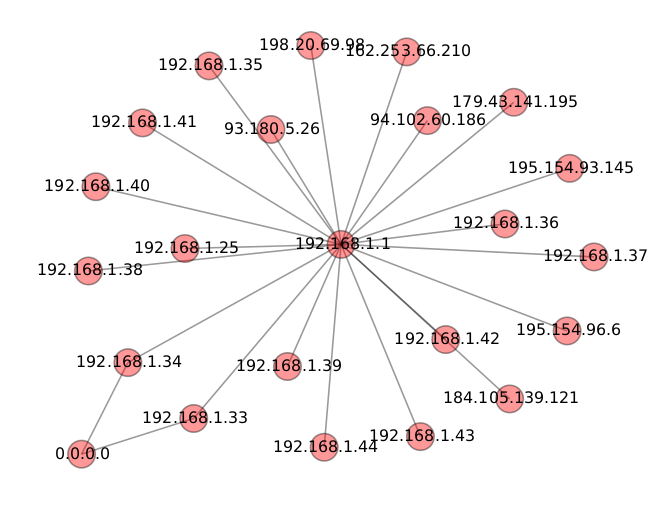
\includegraphics[scale=.6]{resultados/casa/conectividadNX.png}
		  \caption{Grafo de conectividad en la casa}
	\end{center}
\end{figure}
	
En el caso de la casa familiar sabemos que la direcci\'on del router
es 192.168.1.1 y que 192.168.1.35 pertenece al dispositivo que m\'as tiempo estuvo
prendido, el mismo es una notebook. Podemos apreciar que la ip del
router es de las que aparece con mayor frecuencia en los campos SRC (fig \emph{a}) 
o DST (fig \emph{b}), mientras que la notebook solo aparece un alto n\'umero de 
veces en DST. 

En la \emph{Figura 1} representamos la red como un grafo, en el mismo los
nodos son dispositivos y las aristas representan que existi\'o al menos
un paquete que ten\'ia a alguno de ellos como $src$ y al otro como $dst$.
Podemos ver que la red qued\'o representada con el router en el centro.
La \emph{Figura 2} presenta esta misma informaci\'on
pero con mayor detalle, nuevamente los nodos son dispositivos, pero en este
caso las aristas son dirigidas, cada arista representa la cantidad de veces
que el nodo origen envi\'o un paquete ARP al nodo destino.

\begin{figure}[H]
	\center
	\begin{subfigure}{0.43\textwidth}
		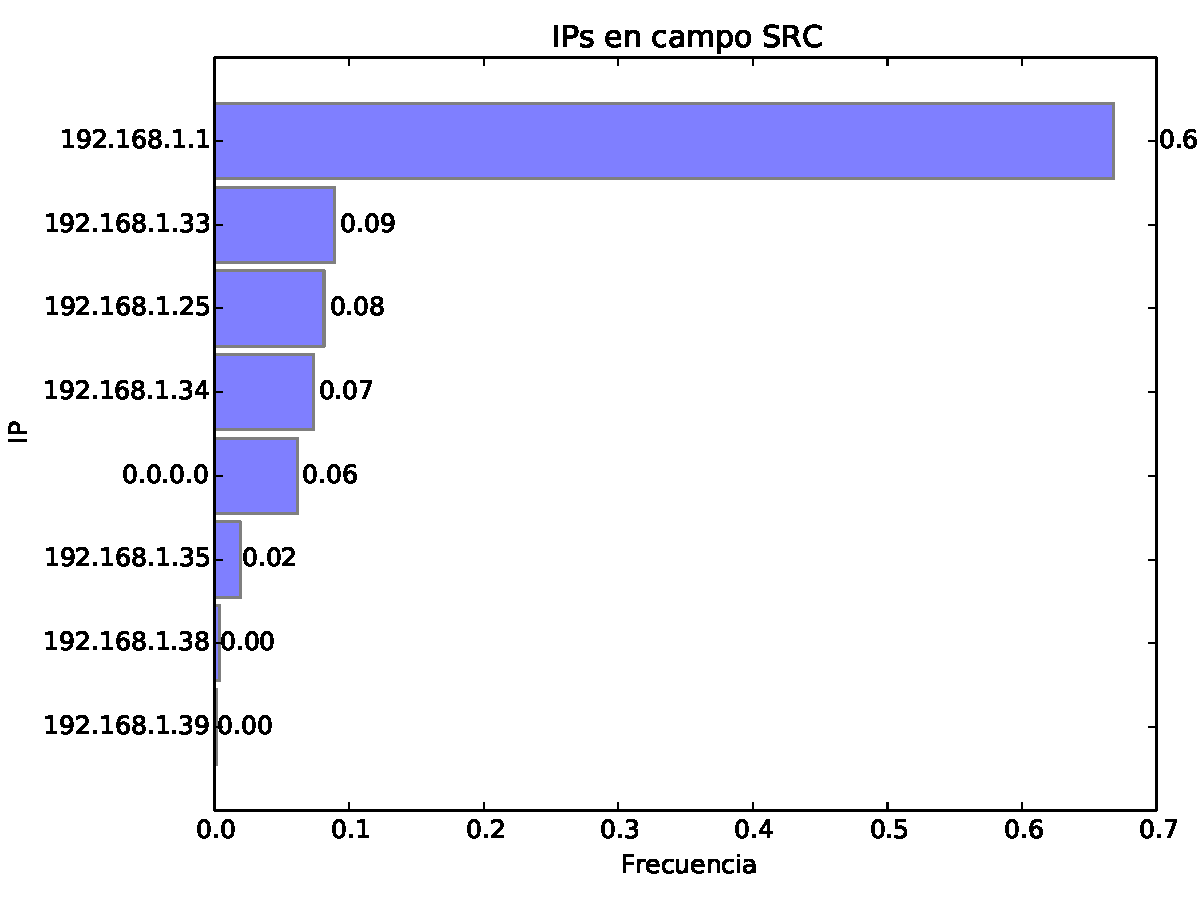
\includegraphics[width=1.0\textwidth]{resultados/casa/ipsSrc_1_6805902069.pdf}
		\caption{a. Estimaci\'on de la probabilidad de cada s\'imbolo en modelo SRC}
	\end{subfigure}
	~
	\begin{subfigure}{0.43\textwidth}
		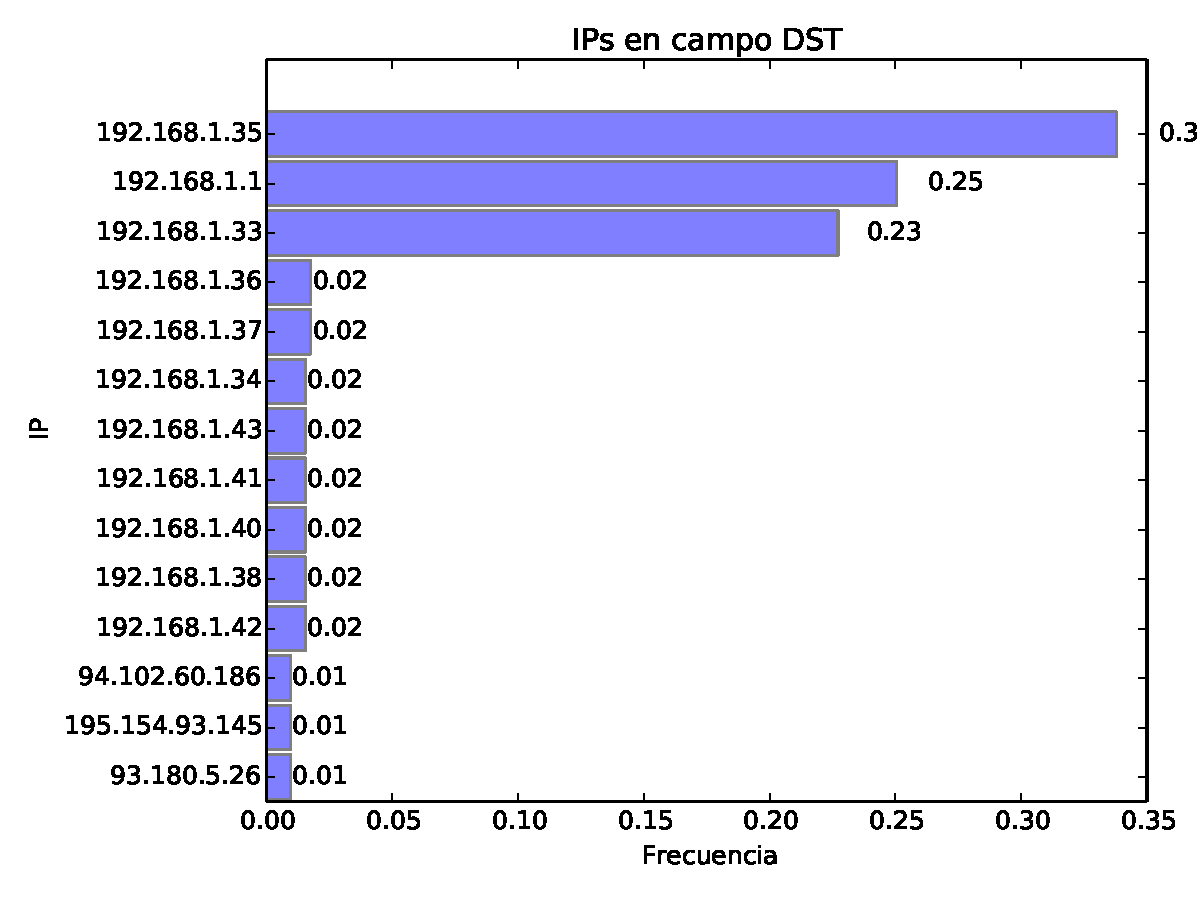
\includegraphics[width=1.0\textwidth]{resultados/casa/ipsDst_2_67355481854.pdf}
		\caption{b. Estimaci\'on de la probabilidad de cada s\'imbolo en modelo DST}
	\end{subfigure}
\end{figure}

La entrop\'ia fue: $1.68$ para el modelo $SRC$ y $2.67$ para el modelo DST.
Teniendo en cuenta que se vieron 23 ips asumimos que existen 23 s\'imbolos
posibles para cada fuente, con lo cual podemos calcular el l\'imite
superior para la entrop\'ia de estos modelos, la misma es $log_2(23)=4.52$, lo 
cual hace que las entrop\'ias normalizadas sean aprox. $0.37$ para $SRC$ y 
$0.59$ para $DST$. Esto indica que es mas probable encontrar la mismas 
IP enviando siempre paquetes, mientras que las IP que reciben la mayor
cantidad de paquetes son varias. Lo que ya se ve\'ia reflejado en los gr\'aficos
\emph{a y b} donde el router es el \'unico que posee una frecuencia de
env\'io 6 veces superior a todo el resto de los nodos, por otro lado en $DST$
son tres los nodos en esta situaci\'on.

Cabe destacar algo interesante que sucedi\'o, aparecieron paquetes ARP que
pose\'ian direcciones que no pertenecian a la red local.


\begin{figure}[!h]
	  \hspace{-5em}
	  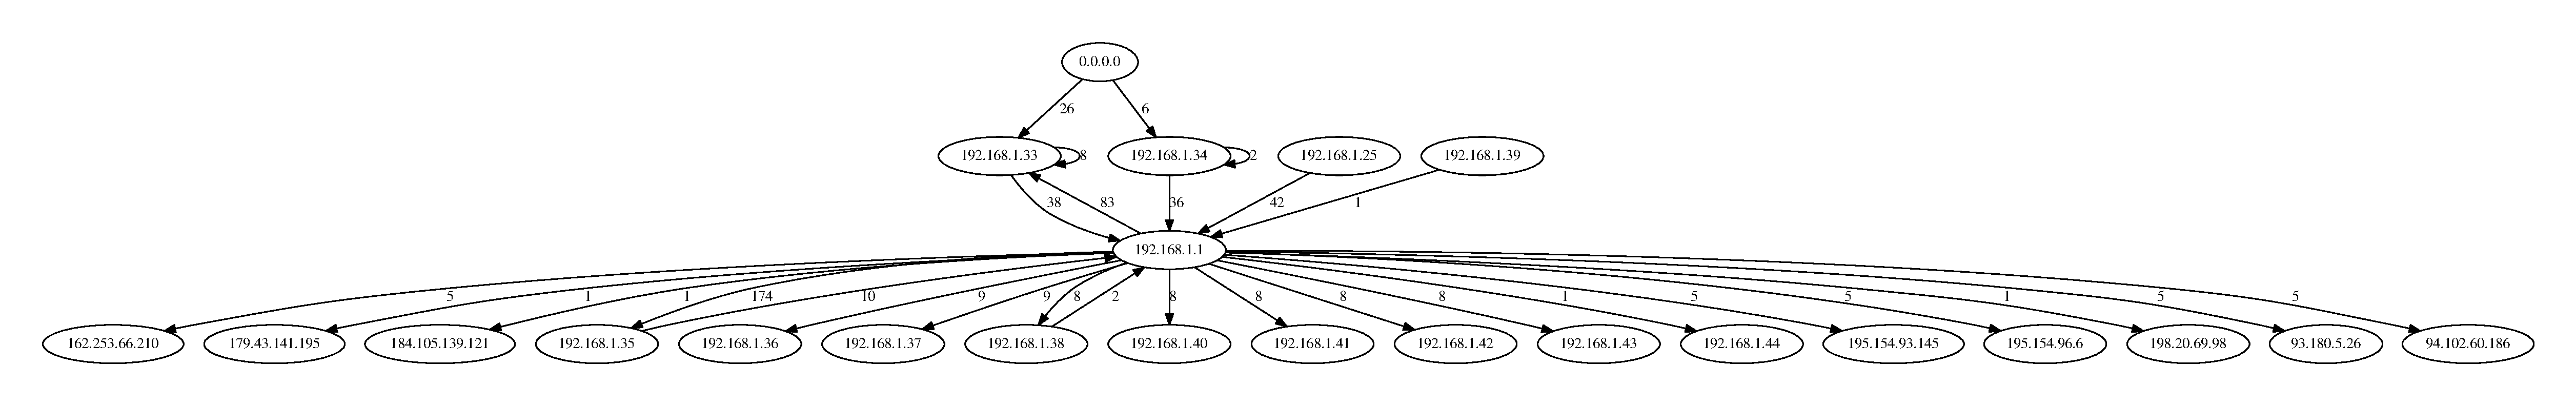
\includegraphics[scale=0.25]{resultados/casa/conectividad.pdf}
	  \caption{Intercambio de paquetes ARP en la casa}
	  \label{fig:contra1}
\end{figure}


\subsection{Empresa}

\begin{figure}[!h]
	\begin{center}
		  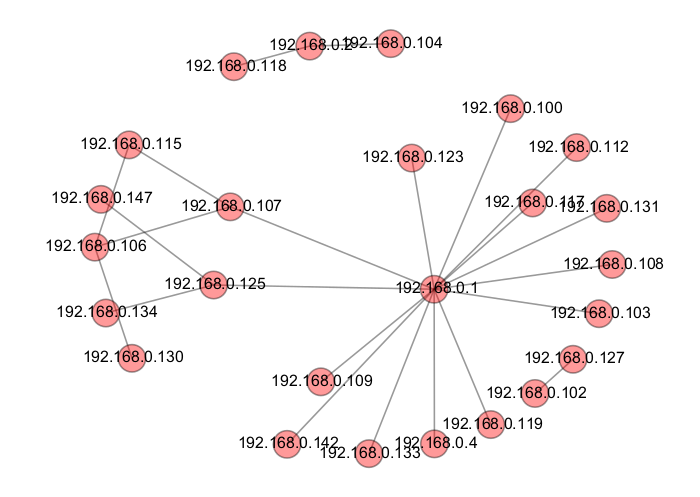
\includegraphics[scale=0.6]{resultados/empresa/conectividadNX.png}
		  \caption{Grafo de conectividad en la empresa}
		  \label{fig:contra1}
	\end{center}
\end{figure}

Al sniffear la empresa se vieron en total 40 ips distintas, para poder
visualizar los datos nos quedamos solo con los 23 pares de nodos que 
mayor intercambio de paquetes ARP tuvieron entre ellos. 
Nuevamente representamos la red como grafos (\emph{Figuras 4 y 5}), 
siguiendo los mismos procedimientos que en el caso anterior. 
Podemos ver que nuevamente el router aparece en el centro de los grafos,
aunque es posible observar una interacción mucho mayor 
entre distintos pares hosts, y no únicamente entre cada uno de estos y el
router.

\begin{figure}[H]
	\center
	\begin{subfigure}{0.43\textwidth}
		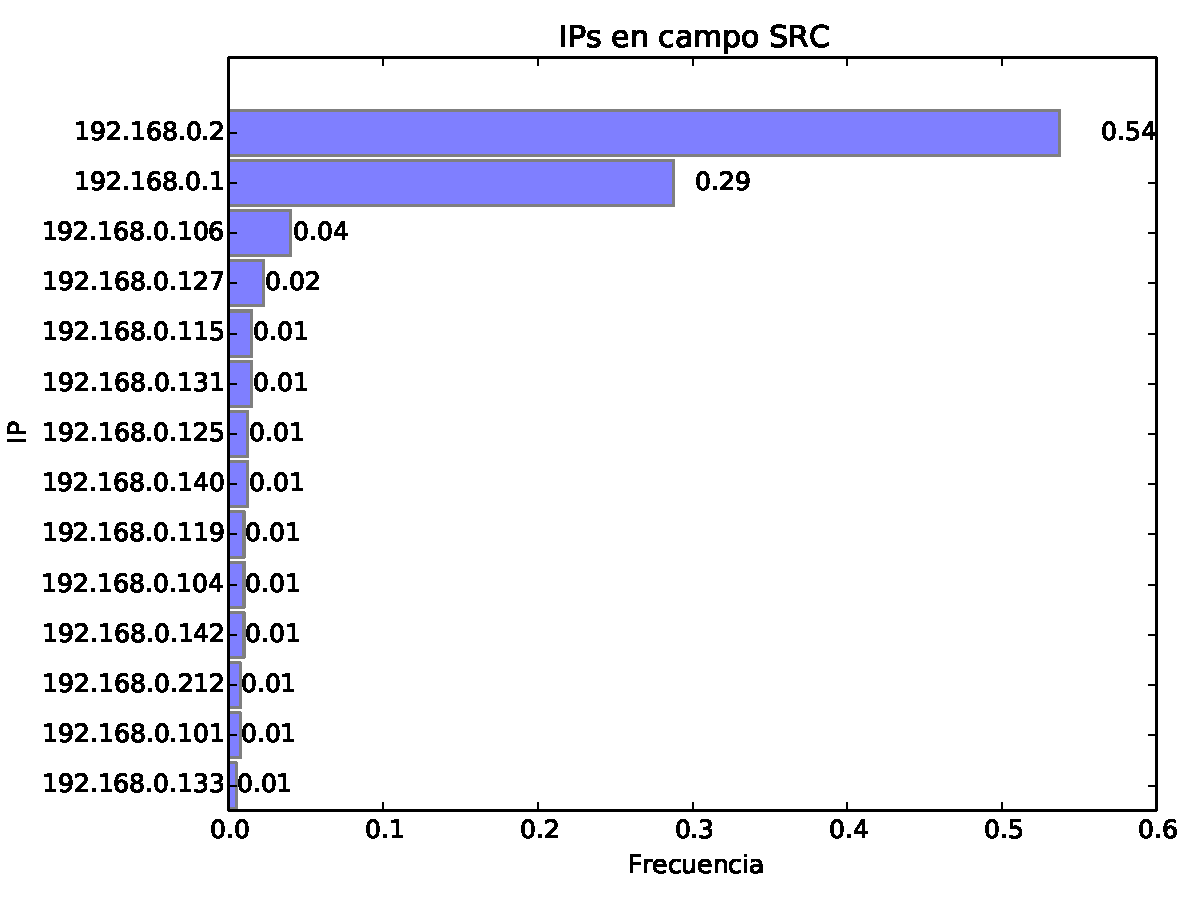
\includegraphics[width=1.0\textwidth]{resultados/empresa/ipsSrc_2_05542931604.pdf}
		\caption{c. Estimaci\'on de la probabilidad de cada s\'imbolo en modelo SRC}
	\end{subfigure}
	~
	\begin{subfigure}{0.43\textwidth}
		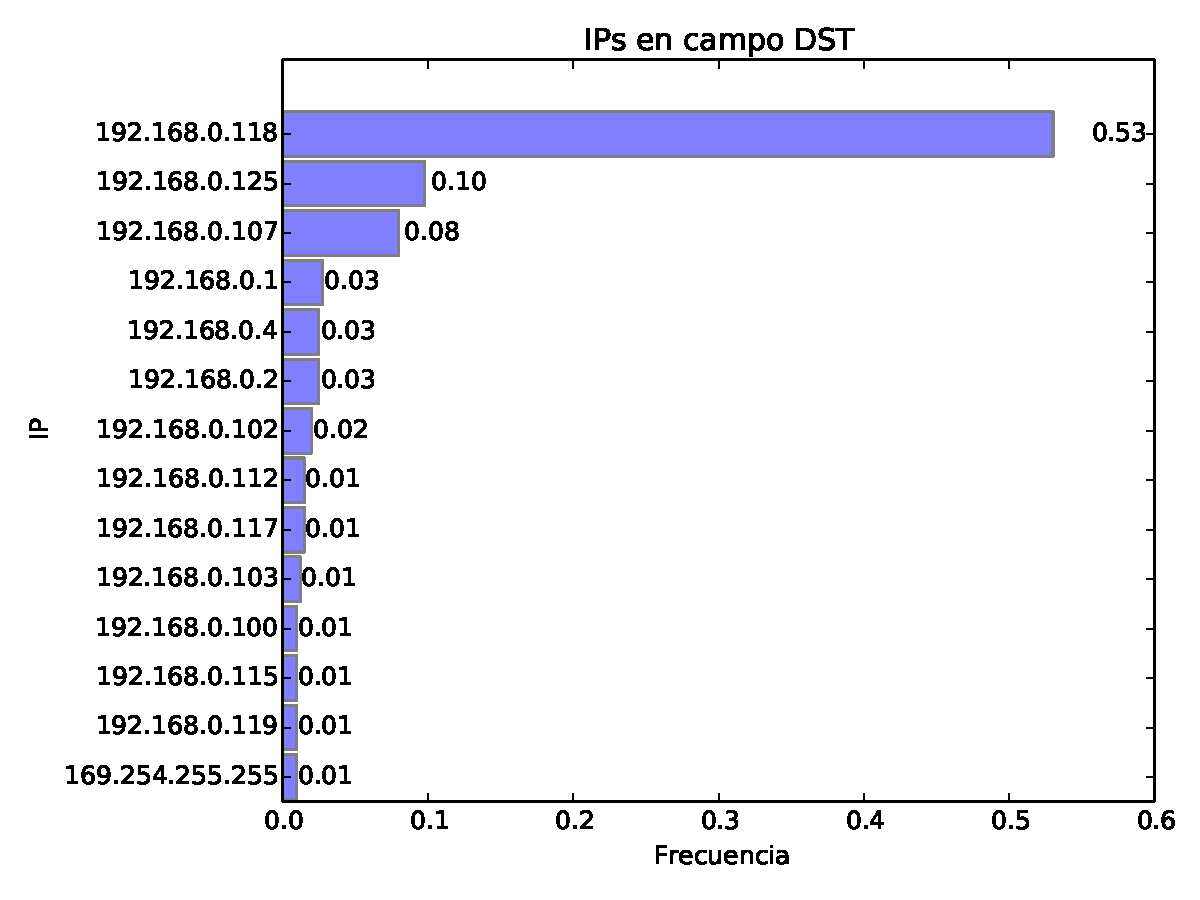
\includegraphics[width=1.0\textwidth]{resultados/empresa/ipsDst_2_99926622579.pdf}
		\caption{d. Estimaci\'on de la probabilidad de cada s\'imbolo en modelo DST}
	\end{subfigure}
\end{figure}

El valor de la entropía para el modelo SRC es $2.05$. El valor de la entropía
para el modelo DST es $2.99$. Teniendo en cuenta que se vieron 40 ips, 
asumimos que las fuentes poseen 40 s\'imbolos, lo cual nos permite 
calcular la entrop\'ia maxima ($log_2(40)=5.32$) lo cual normaliza las 
entropias a $0.38$ y $0.56$. Nuevamente el modelo SRC posee un valor mayor.

En el gráfico de barras del modelo SRC (gr\'afico \emph{c}) el router juega
un papel relevante
ya que es el segundo símbolo con mayor cantidad de emisión de paquetes. Es
interesante mencionar que el nodo con mayor cantidad de paquetes enviados, 
cuya ip es 192.168.0.2, corresponde a un servidor apache. 
El resto de los nodos que aparecen en el gráfico corresponden a notebooks
y celulares conectados a la red, ya a partir del quinto elemento aparecen
con una frecuencia de aparici\'on hasta 50 veces mas baja.

En el gráfico de barras del modelo DST (gr\'afico \emph{d}) es en donde se nota
la mayor cantidad de diferencias. El router no se corresponde con ninguno de los
3 nodos con mayor cantidad de paquetes recibidos:

\begin{itemize}
    \item 192.168.0.118 corresponde a una notebook
    \item 192.168.0.125 corresponde a un servidor apache
    \item 192.168.0.107 corresponde a un servidor apache
\end{itemize}

Recién aparece en la cuarta posición, con una cantidad de paquetes recibidos
considerablemente menor a los primeros. En esta red en particular los
dispositivos se envían paquetes who-has entre ellos en mayor medida, y hacia
los servidores en vez de hacia el router. A su vez, podemos ver que en este
caso son ocho las ips que poseen desde el doble hasta 50 veces mas frecuencia
de aparici\'on. Suponemos que por esto la entrop\'ia de este modelo es mas alta.

\begin{figure}[H]
	\center
	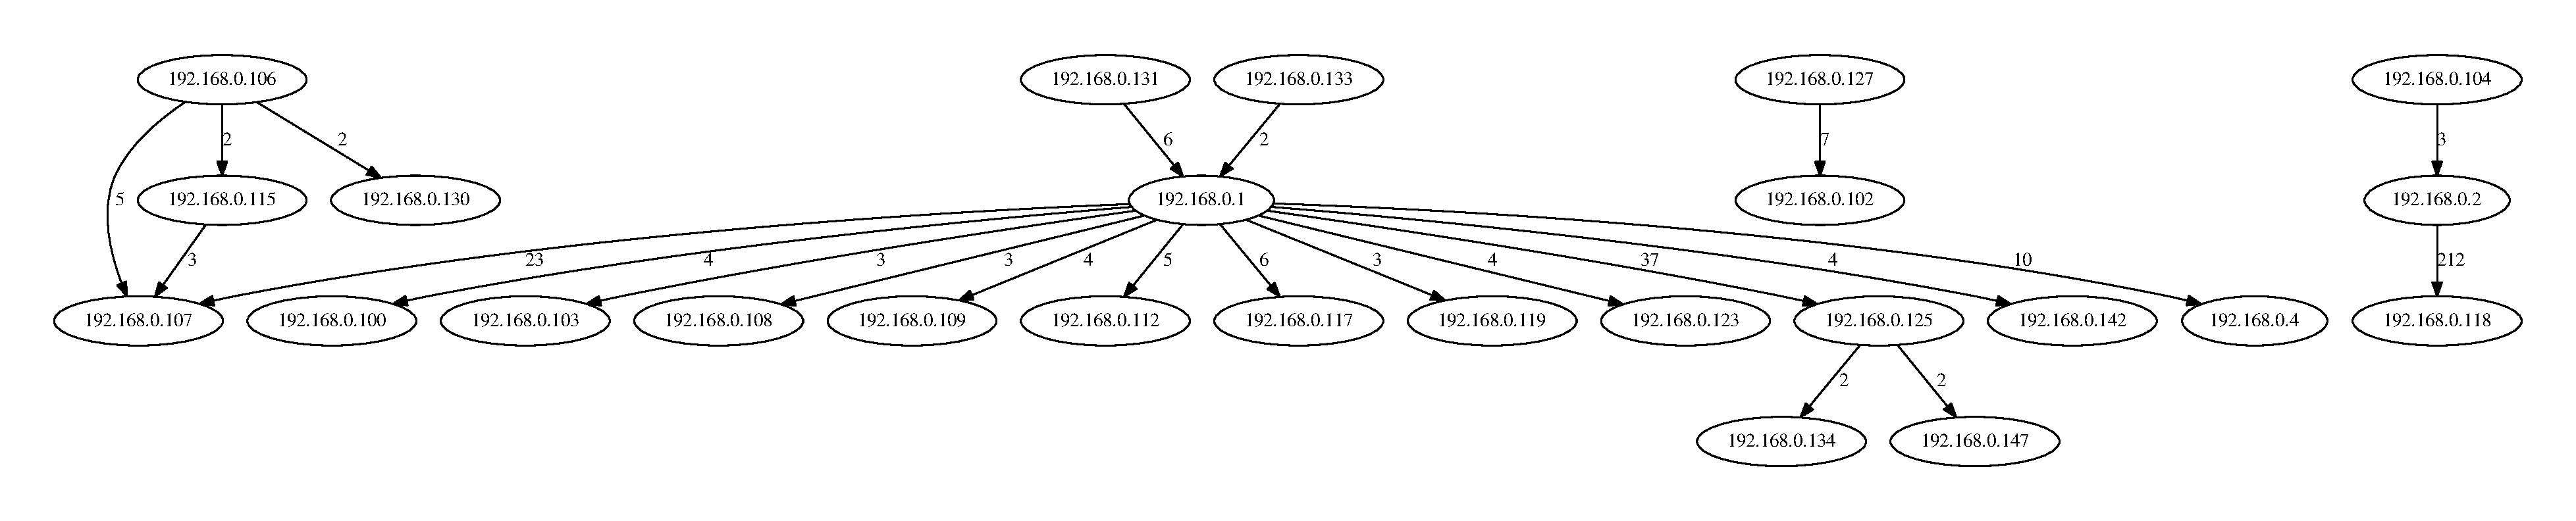
\includegraphics[scale=0.3]{resultados/empresa/conectividad.pdf}
	\caption{Intercambio de paquetes ARP en la empresa}
\end{figure}



\subsection{Starbucks}

\begin{figure}[h!]
	\begin{center}
		  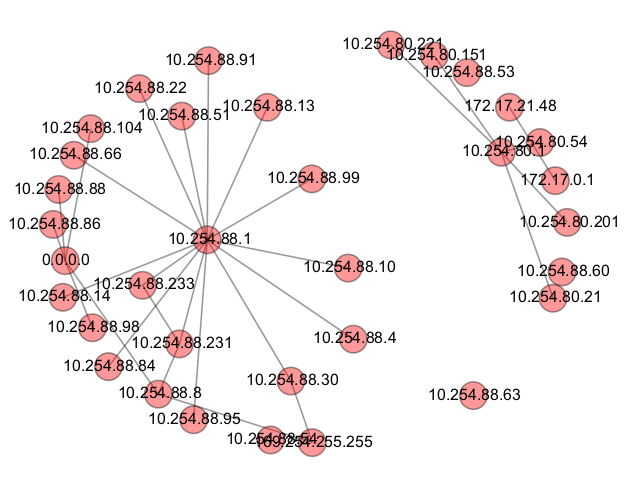
\includegraphics[scale=.6]{resultados/starbucks/conectividadNX.png}
		  \caption{Grafo de conectividad en Starbucks}
		  \label{fig:contra1}
	\end{center}
\end{figure}


Para el caso de la red abierta disponible en Starbucks se recopil\'o
informaci\'on de 200 nodos en total, la \emph{Figura 7} fue 
creada con solo 40 de ellos, en caso de agregar m\'as nodos se notar\'ia
que todos est\'an conectados que el nodo 10.254.88.1. 
A su vez posee una alta frecuencia de aparici\'on en ambos
modelos. Esto ser\'ia el comportamiento esperado del router de la red
10.254.88.0/24. Asumimos que \'esta es la direcci\'on de la red puesto que 
la mayor\'ia de las IPs de los paquetes capturados difieren en el \'ultimo octeto.
Por otro lado, podemos ver que la segunda direcci\'on con mayor frecuencia en DST
fue 10.254.80.1, seguida por 10.254.88.8. Suponemos que $88.8$ es la pc del lugar
dada la ip baja, y la cantidad de apariciones. Por otro lado, no sabemos que es
$80.1$ dado que parece formar una red aparte de la sniffeada.

\begin{figure}[H]
	\center
	\begin{subfigure}{0.43\textwidth}
		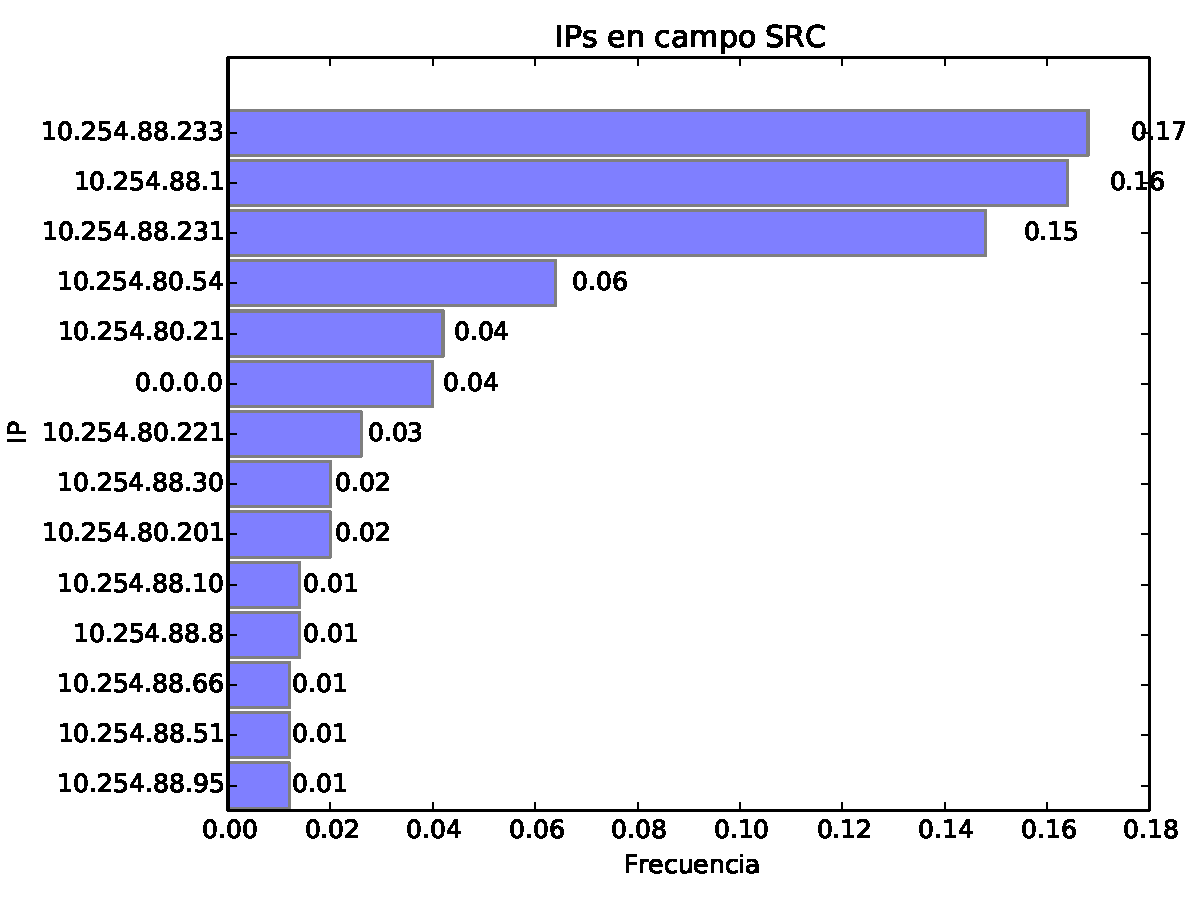
\includegraphics[width=1.0\textwidth]{resultados/starbucks/ipsSrc_4_6187931499.pdf}
		\caption{e. Estimaci\'on de la probabilidad de cada s\'imbolo en modelo SRC}
	\end{subfigure}
	~
	\begin{subfigure}{0.43\textwidth}
		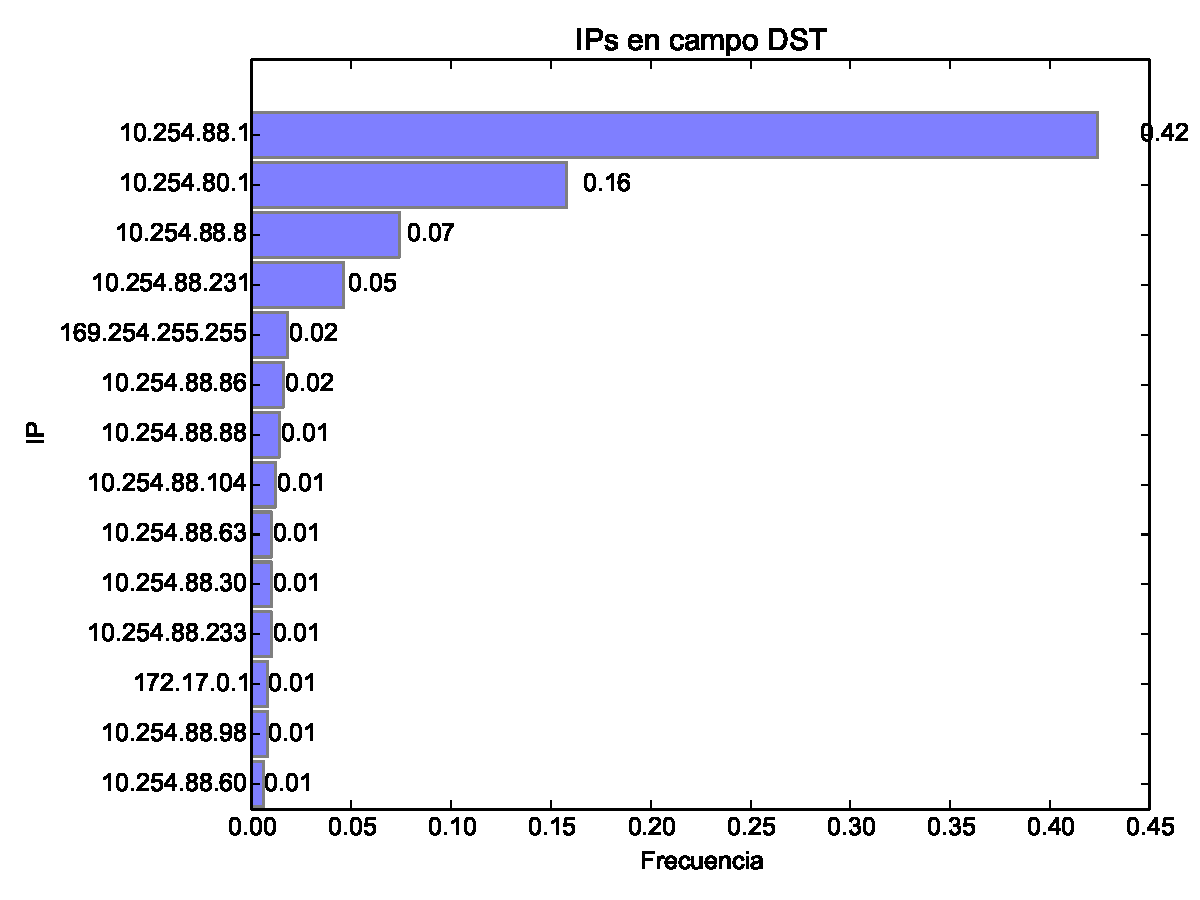
\includegraphics[width=1.0\textwidth]{resultados/starbucks/ipsDst_3_76848714287.pdf}
		\caption{f. Estimaci\'on de la probabilidad de cada s\'imbolo en modelo DST}
	\end{subfigure}
\end{figure}

La entrop\'ia fue: $4.61$ para el modelo $SRC$ y $3.76$ para el modelo
DST. La entrop\'ia m\'axima dado los 200 s\'imbolos es $log_2(200)=7.64$,
por lo que normalizadas quedarían $SRC=0.60$ y $DST=0.48$. Esto es 
consistente con los graficos \emph(e y f) donde las frecuencias de aparici\'on
de cada s\'imbolo decaen mucho m\'as r\'apidamente en DST.

Nuevamente entre los paquetes capturados volvieron a aparecer direcciones que
no parecieran pertenecer a la red local, resultando sumamente interesante el caso
de 10.254.80.1


\subsection{Entrepiso}

\begin{figure}[h!]
    \center
    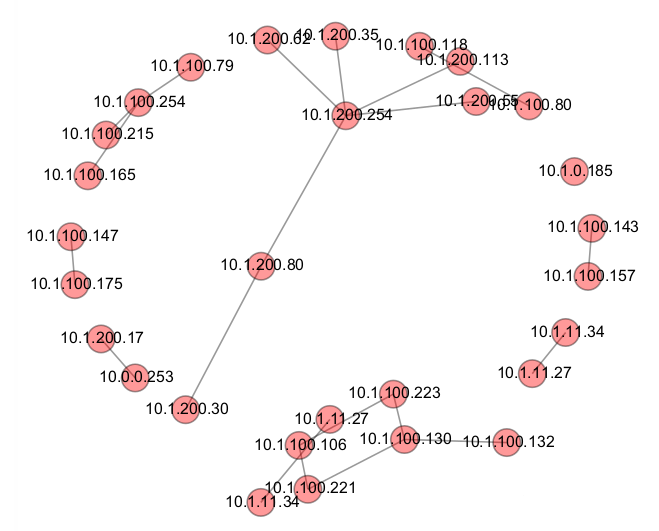
\includegraphics[scale=0.6]{resultados/entrepiso/conectividadNX.png}
    \caption{Grafo de conectividad en la red Entrepiso}
\end{figure}

En el caso del entrepiso se detectaron 205 ips, lamentablemente la forma en que
las mismas se comunicaron entre si hizo imposible el graficar una representaci\'on
adecuada con las herramientas que usamos. La \emph{Figura 9} muestra
varios subgrafos conexos, donde se destacan los nodos: 10.1.100.254, 10.1.200.30
y 10.1.200.254. Por las direcciones IP $200.254$ y $100.254$ parecieran ser routers.
La entrop\'ia fue: $4.25$ para el
modelo $SRC$ y $4.90$ para el modelo DST. Estos valores normalizados son: 
$0.55$ y $0.63$ respectivamente, ambos son valores muy altos. 
Podemos ver esto reflejado en los gr\'aficos \emph{g y h}, donde las diferencias
en frecuencias entre los nodos no es tan grande como en los casos vistos hasta
ahora.

A su vez, si no fuera por la \emph{Figura 8} no podriamos buscar un
candidato tan claro a router, ya que $200.254$ y $100.254$ aparecen reci\'en
en cuarto y quinto lugar para SRC, mientras que aparecen en quinto y decimo 
lugar para DST.

Una vez mas aparecieron direcciones sueltas, como es por ej: 10.1.11.254.

\begin{figure}[H]
	\center
	\begin{subfigure}{0.43\textwidth}
		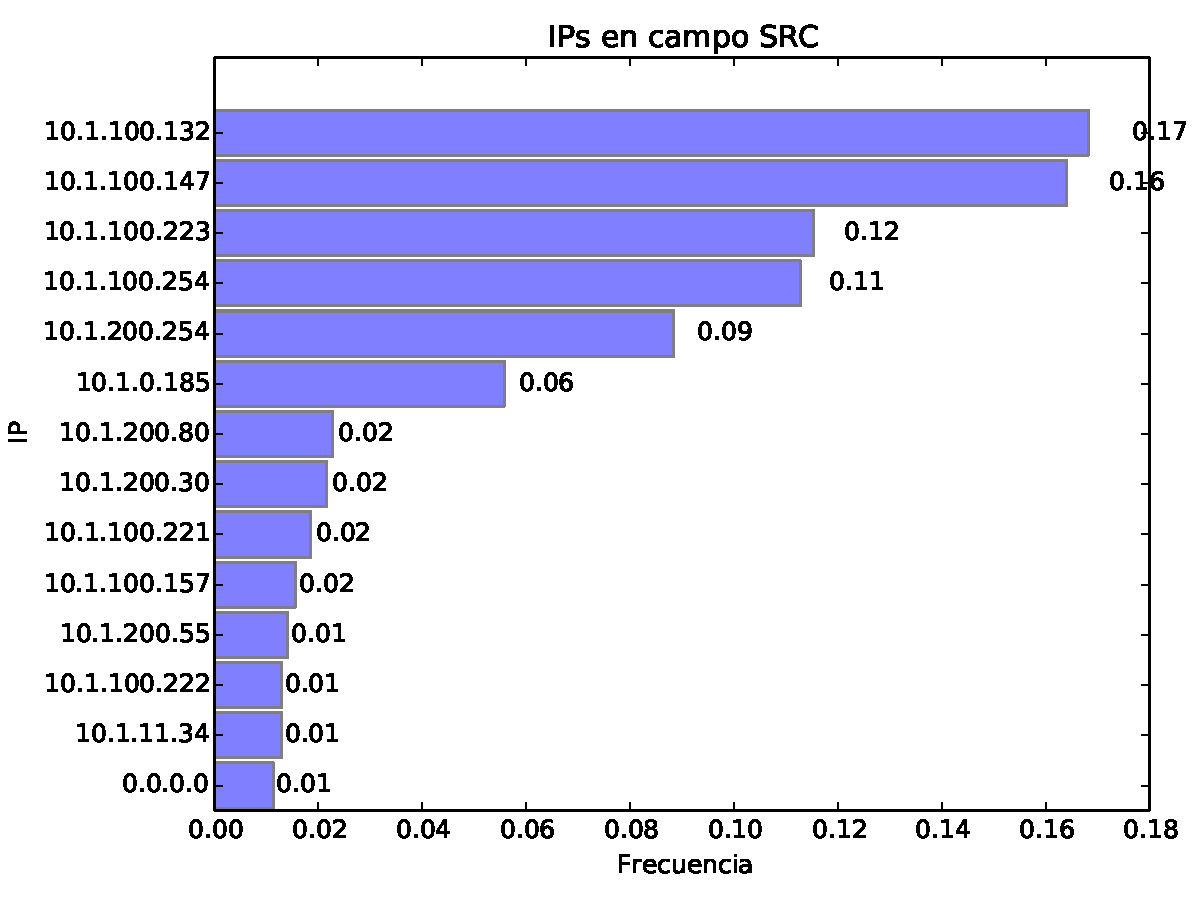
\includegraphics[width=1.0\textwidth]{resultados/entrepiso/ipsSrc_4_25991830161.pdf}
		\caption{g. Estimaci\'on de la probabilidad de cada s\'imbolo en modelo SRC}
	\end{subfigure}
	~
	\begin{subfigure}{0.43\textwidth}
		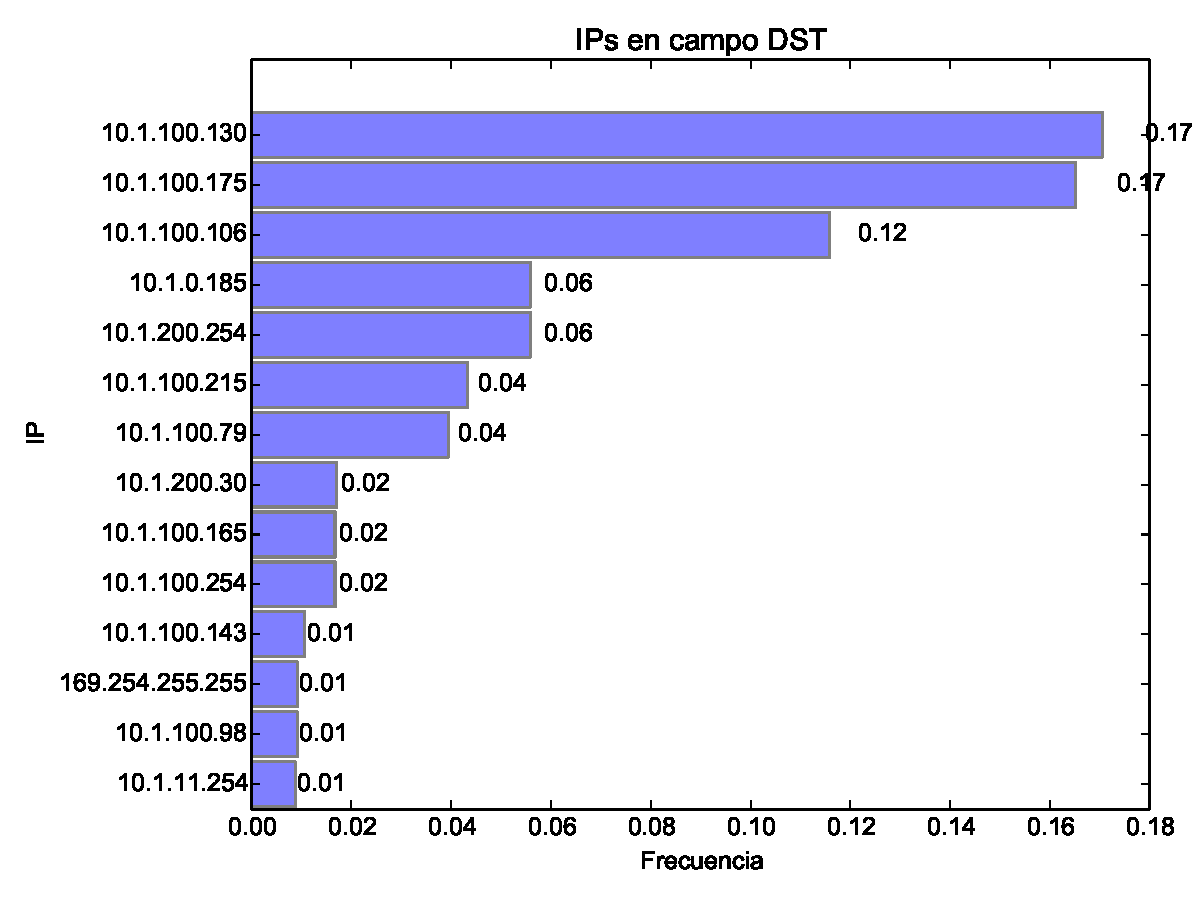
\includegraphics[width=1.0\textwidth]{resultados/entrepiso/ipsDst_4_90633854055.pdf}
		\caption{h. Estimaci\'on de la probabilidad de cada s\'imbolo en modelo DST}
	\end{subfigure}
\end{figure}


\subsection{Discusi\'on}

        En todas las redes sucedi\'o que aparecieran direcciones ip que se supone
no pertenecen a la misma. 

        En algunos casos apareci\'o la direcci\'on 169.254.255.255. Investigando
encontramos que es utilizada como broadcast por DHCP que es un protocolo de 
configuraci\'on autom\'atica de par\'ametros de red tales como direcciones IP
para interfaces y servicios.

        La direcci\'on 0.0.0.0 es el est\'andar para \emph{broadcastear} dentro
de una red local.

        Por otra parte, el resto de las direcciones IP que aparecen pueden deberse
a que los routers posean la opci\'on de \emph{Proxy ARP} habilitada, cosa que tiene 
mucho sentido en el caso del Entrepiso por ejemplo.

        Es posible que las direcciones que aparecen con mayor frecuencia en el grafo
de pedidos ARP correspondan los dispositivos que estabam m\'as activos durante el periodo
de tiempo que se hizo el sniffing.

